
%(BEGIN_QUESTION)
% Copyright 2006, Tony R. Kuphaldt, released under the Creative Commons Attribution License (v 1.0)
% This means you may do almost anything with this work of mine, so long as you give me proper credit

Calculate the output voltage of this bridge circuit at the following RTD temperatures (assume the use of a 100 $\Omega$ RTD with an American alpha value).

$$\includegraphics[width=15.5cm]{i00690x01.eps}$$

\begin{itemize}
\item{} $V_{out}$ = \underbar{\hskip 50pt} at $T$ = -20$^{o}$ C
\vskip 5pt
\item{} $V_{out}$ = \underbar{\hskip 50pt} at $T$ = 70$^{o}$ C
\vskip 5pt
\item{} $V_{out}$ = \underbar{\hskip 50pt} at $T$ = 200$^{o}$ C
\end{itemize}

\underbar{file i00690}
%(END_QUESTION)





%(BEGIN_ANSWER)

\begin{itemize}
\item{} $V_{out}$ = \underbar{\bf -2.04 mV} at $T$ = -20$^{o}$ C
\vskip 5pt
\item{} $V_{out}$ = \underbar{\bf 6.032 mV} at $T$ = 70$^{o}$ C
\vskip 5pt
\item{} $V_{out}$ = \underbar{\bf 14.08 mV} at $T$ = 200$^{o}$ C
\end{itemize}


%(END_ANSWER)





%(BEGIN_NOTES)


%INDEX% Measurement, temperature: RTD

%(END_NOTES)


